
\section{\en{Welcome}\de{Willkommen}}

\en{I present a way of looking at the world here. That way or
idea is not something that can be proven. But some of the
fruits it contains might be considered for tending to, grow
and become part of existing systems of thought.}%
\de{Ich präsentiere hier eine Art, die Welt anzuschauen. Dieser
Weg oder diese Idee ist nicht etwas, das bewiesen werden
kann. Aber einige der Früchte, die sie enthält, könnten in
Betracht gezogen werden, sie zu pflegen, wachsen zu lassen
und Teil existierender Denksysteme zu werden.}

\en{Just read all sections sequentially, like reading chapters
in a book,\hspace{-0.1ex}{\raisebox{0.25ex}{\smaller *}} and take your time, or go to individual articles
at ‘\cometartemis’ for every- and nothing…}%
\de{Einfach alle Sektionen der Reihe nach lesen, wie beim
Lesen von Kapiteln in einem Buch,\hspace{-0.1ex}{\raisebox{0.3ex}{\smaller *}} und sich Zeit dabei lassen,
oder zu ‘\cometartemis’ für Artikel über alles und nichts…}

\en{I am a physicist ($^*$\,1966 in Zürich, Switzerland) and am
doing this as a hobby.}%
\de{Ich bin Physiker ($^*$\,1966 in Zürich, in der Schweiz) und
mache das als ein Hobby.}

\vspace{3mm}
\noindent
Alain Stalder

\noindent
\hspace{20mm}%
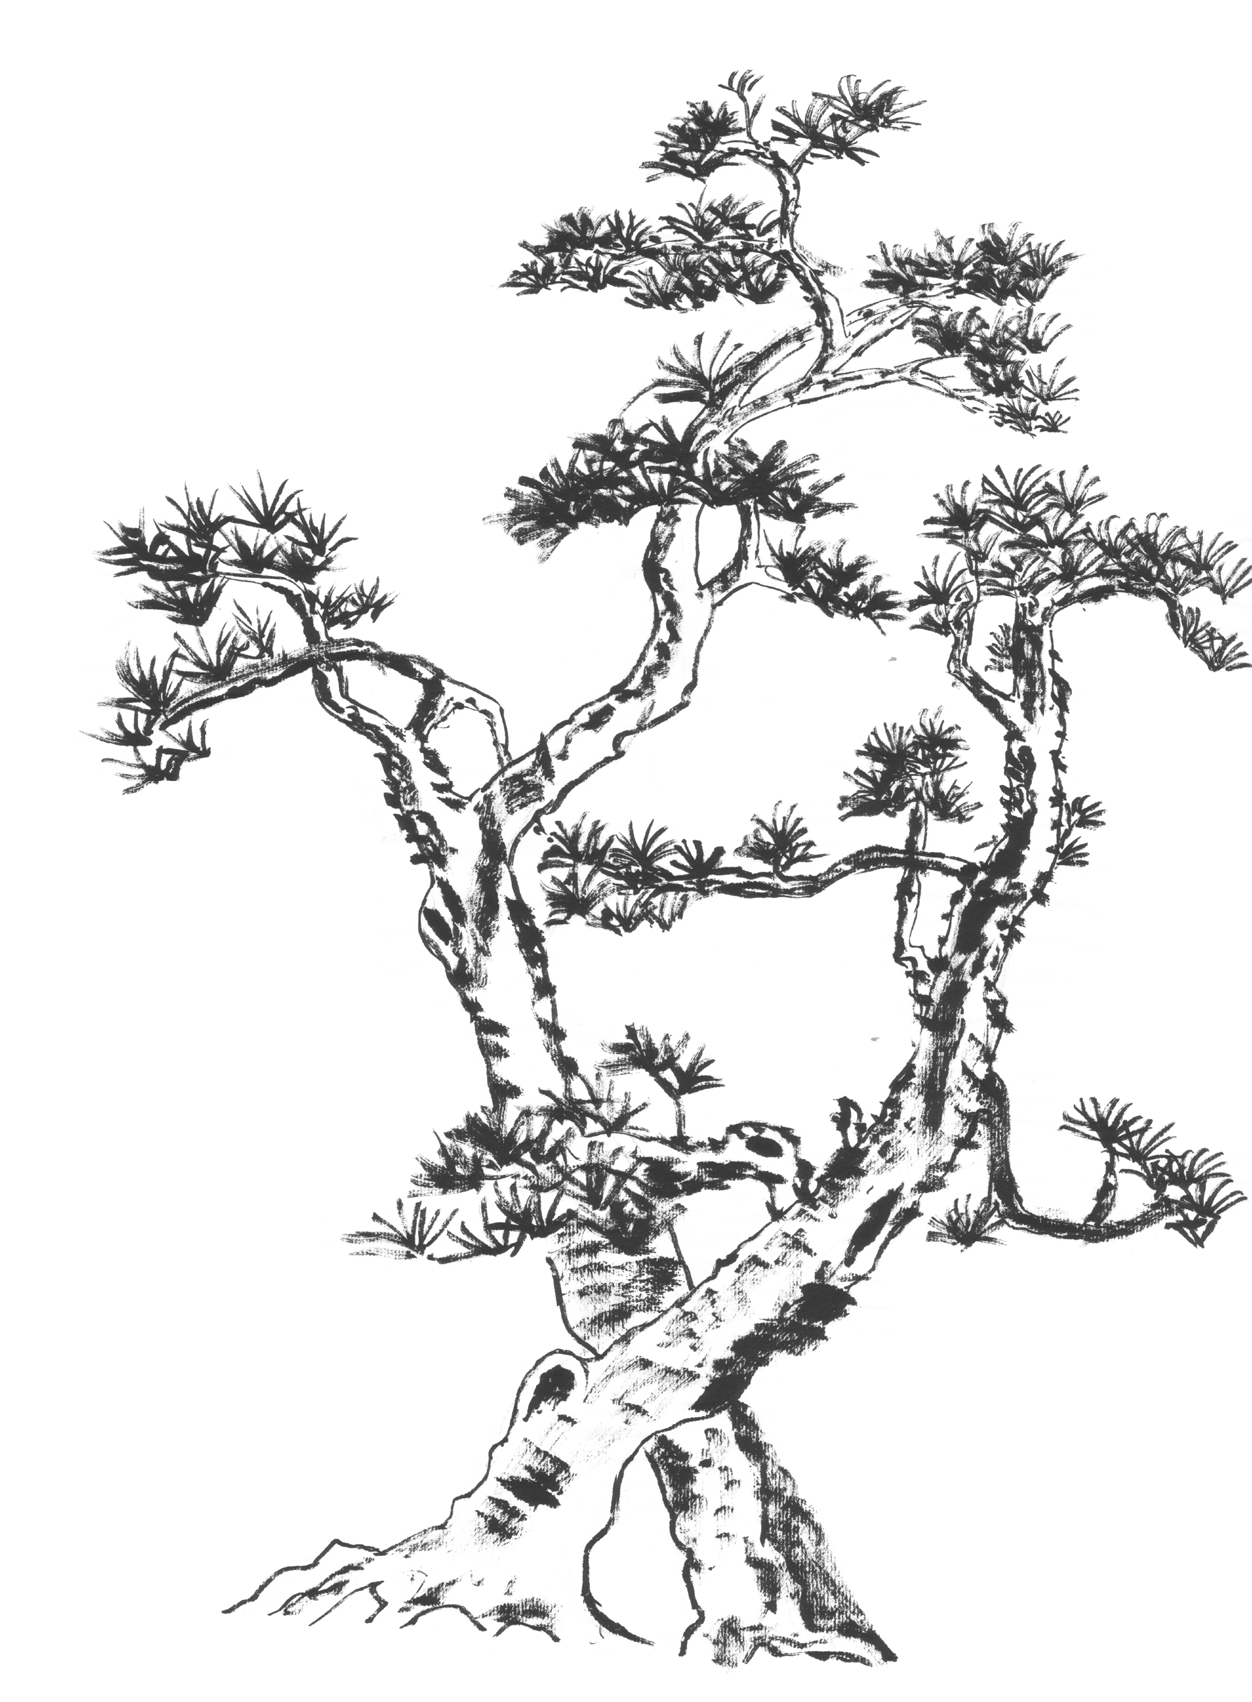
\includegraphics[scale=0.1198]{i-fuse.png}

\vspace{10mm}
\noindent
\en{\small {\raisebox{0.15ex}{\smaller *}} If you are not much of a researcher, see ‘Series’ instead, for
an emerging series of accessible pocket books, already while
writing for free as pdfs, plus the first tome contains the current
core web pages conveniently in a {\color{xphi}single pdf}\,!}%
\de{\small {\raisebox{0.15ex}{\smaller *}} Wer nicht gross Forscher ist, siehe stattdessen ‘Reihe’, für
mit der Zeit entstehende, zugängliche Taschenbüchlein, bereits
während des Schreibens gratis als pdfs, plus der erste Band
enthält die aktuellen Webseiten bequem in einem {\color{xphi}einzigen pdf}\,!}

